\documentclass[10pt,a4paper]{article}
\usepackage[T1]{fontenc}
\usepackage[utf8]{inputenc}

\usepackage{etex}

\usepackage[english]{babel}

\usepackage{amsmath,amssymb}
\usepackage{amsthm,thmtools}
\usepackage{mathrsfs}
\usepackage{MnSymbol}
\numberwithin{equation}{section}
\declaretheorem[sibling=equation]{theorem}
\declaretheorem[sibling=equation]{proposition}
\declaretheorem[sibling=equation]{lemma}
\declaretheorem[sibling=equation]{definition}
\declaretheorem[sibling=equation]{fact}
\declaretheorem[sibling=equation,style=remark]{remark}
\declaretheorem[sibling=equation,style=remark]{idea}
\declaretheorem[sibling=equation,style=remark]{observation}
\declaretheorem[sibling=equation]{conjecture}
\declaretheorem[sibling=equation]{notation}
\declaretheorem[sibling=equation]{example}
\declaretheorem[sibling=equation,style=remark]{exercise}
\newenvironment{solution}{}{}

\usepackage{enumitem}

\usepackage{tikz}
\usepackage{tikz-cd}

\newcommand{\ZZ}{\mathbb{Z}}
\newcommand{\QQ}{\mathbb{Q}}
\newcommand{\RR}{\mathbb{R}}
\newcommand{\CC}{\mathbb{C}}
\newcommand{\FF}{\mathbb{F}}
\newcommand{\Aff}{\mathbb{A}}
\newcommand{\Spec}{\mathrm{Spec}}
\newcommand{\Jac}{\mathrm{Jac}}
\newcommand{\Pic}{\mathrm{Pic}}
\newcommand{\Hom}{\mathrm{Hom}}
\newcommand{\Trop}{\mathrm{Trop}}
\newcommand{\an}{\mathrm{an}}
\newcommand{\val}{\mathrm{val}}
\newcommand{\ord}{\mathrm{ord}}

\newcommand{\chr}{\mathrm{char}}

\newcommand{\nr}{\mathrm{nr}}

\usepackage[usenames,dvipsnames]{pstricks}
\usepackage{epsfig}
\usepackage{graphicx,color}
\usepackage[all]{xy}
\xyoption{poly}

%Preamble by JK (lec10)
% fonts
\usepackage{calrsfs}

\newcommand{\scheme}{\mathcal{X}}
\DeclareMathOperator{\Sp}{sp}
\DeclareMathOperator{\Sk}{Sk}

\renewcommand{\tilde}{\widetilde}
\renewcommand{\bar}{\overline}
%\DeclareMathOperator{\Stab}{{Stab}}
%\newcommand{\f}{\varphi}


%BEGIN TEMP
\newcommand{\mynote}[2]{\noindent
{\bfseries\sffamily\scriptsize#1}
{\small$\blacktriangleright$\textsf{\textsl{#2}}$\blacktriangleleft$}}
\newcommand\JK[1]{\mynote{JK}{{\color[rgb]{0,0.2,0.5} #1}}}
\newcommand\GC[1]{\mynote{GC}{{\color[rgb]{0.5,0.2,0.0} #1}}}
%END TEMP
%End preamble by JK (lec10)

\usepackage{hyperref}
\usepackage{cleveref}

\title{Lecture notes on Berkovich skeleta}
\author{Johannes Nicaise \and Sam Payne}

\begin{document}
\maketitle

\tableofcontents

\section{Lecture 1}

\subsection{Motivation}

To study the geometry of a complex variety $X/\CC$ it is often useful to put it
into a family and to study the other fibres
\[
	f \colon \mathfrak{X} \to \Aff^{1}_{\CC}
\]
such that $X \cong f^{-1}(a)$ for some $a$.

Typical situation: $X$ is smooth and proper over $\CC$. Then one might take
$\mathfrak{X}$ regular, $f$ proper and flat, and such that all singular fibres
of $f$ are strict normal crossings divisors.
(Strict normal crossings divisors means that locally they look like unions of
coordinate hyperplanes.)
\begin{center}
	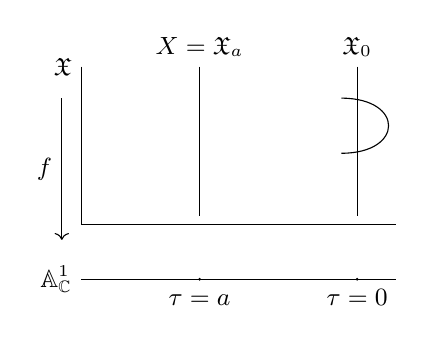
\begin{tikzpicture}[every node/.style={font=\small}]
		\draw (-2,2) node[left] {$\mathfrak{X}$} -- (-2,0) -- (2,0);
		\draw (-2,-.7) node[left] {$\Aff^{1}_{\CC}$} -- (2,-.7);
		\draw[->] (-2.25,1.6) -- node[left] {$f$} (-2.25,-.2);
		\draw (-.5,2) node[above] {$X = \mathfrak{X}_{a}$} -- (-.5,.1);
		\draw (1.5,2) node[above] {$\mathfrak{X}_{0}$} -- (1.5,.1);
		\draw (1.3,1.6) to [controls=+(0:.8) and +(0:.8)] (1.3,0.9);
		\draw[fill] (-.5,-.7) circle (.01) node[below] {$\tau = a\vphantom{0}$};
		\draw[fill] (1.5,-.7) circle (.01) node[below] {$\tau = 0$};
	\end{tikzpicture}
\end{center}
\begin{idea}
	The geometric complexity of $X$ is reflected in the geometric
	complexity of $\mathfrak{X}_{0}$.

	If we want to study the degeneration of the family at a particular
	fibre $\mathfrak{X}_{0}$, we can zoom in around $\mathfrak{X}_{0}$ by
	base changing to $\widehat{\mathcal{O}_{\Aff^{1}_{\CC,0}}} = \CC[[T]]$.

	So we want to study schemes over discrete valuation rings.
\end{idea}

\begin{notation}
	\begin{itemize}
		\item[$R$] discrete valuation ring
		\item[$t$] local uniformizer (i.e., generator of the maximal ideal)
		\item[$k$] residue field (we assume $k = \bar{k}$)
		\item[$K$] fraction field
	\end{itemize}
\end{notation}

\begin{example}
	There are two cases.
	\begin{itemize}
		\item The \emph{equal} characteristic case: $R = k[[t]]$, $K = k((t))$.
		\item The \emph{mixed} characteristic case: $R = \widehat{\ZZ_{p}^{\nr}} = W(\FF_{p})$, $K = \widehat{\QQ_{p}^{\nr}}$, $t = p$. (In general $R$ is a finite extension of $W(k)$.)
	\end{itemize}
\end{example}
The geometric picture corresponding to this is
\begin{itemize}
	\item[$\Spec(R)$] ``small disk around $0 \in \CC$''
	\item[$t$] ``coordinate on this disk''
	\item[$\Spec(K)$] ``small punctured disk around $0 \in \CC$''
\end{itemize}

Let $X$ be a smooth proper geometrically connected variety over $K$.
Geometrically we can think of a family of connected smooth proper varieties
over a punctured disk.
\begin{definition}
	A \emph{model for $X$ over $R$} is a proper and flat $R$-scheme $\mathfrak{X}$ together with an isomorphism $\mathfrak{X}_{K} \to X$.

	A morphism of models $\mathfrak{Y} \to \mathfrak{X}$ is an $R$-morphism such that
	\[
		\begin{tikzcd}[column sep=small]
			\mathfrak{Y}_{K} \ar{rr} \drar[near start,sloped]{\sim}
			&& \mathfrak{X}_{K} \dlar[near start,swap,sloped]{\sim} \\
			& X
		\end{tikzcd}
	\]
	commutes.
\end{definition}
Note: There exists at most one morphism from $\mathfrak{Y}$ to $\mathfrak{X}$.
If such a morphism exists, we say that $\mathfrak{Y}$ dominates $\mathfrak{X}$.
We say that $\mathfrak{X}$ is an \emph{snc-model} if $\mathfrak{X}$ is regular
and $\mathfrak{X}_{k}$ is a strict normal crossings divisor, i.e., for every $x
\in \mathfrak{X}$, there exists a regular system of local parameters
\emph{(i.e., a basis of the Zariski tangent space)} $(Z_{1}, \ldots Z_{d})$ and
a unit $u$ in $\mathcal{\mathfrak{X},x}$ such that $t = uZ_{1}^{N_{1}} \cdots
Z_{d}^{N_{d}}$ for some $N_{i} \ge 0$. We say that $\mathfrak{X}$ is an
\emph{nc-model} if $\mathfrak{X}$ is regular and $\mathfrak{X}_{k}$ is a normal
crossings divisor, i.e., an snc-divisor for the étale topology. This ``allows
for self-intersections''.
\begin{center}
	\begin{tikzpicture}[every node/.style={font=\small}]
		\draw (0,0) to [controls=+(110:3) and +(250:3)] (0,1);
		\path (0,.5) node[right] {nc, but not snc};

		\draw[->] (-.5,-1.2) -- node[right] {étale} (-.5,-.4);

		\begin{scope}[yshift=-2.5cm]
			\draw (0,0) to [controls=+(180:1) and +(180:1)] (0,1);
			\draw (0,.1) to [controls=+(200:2) and +(160:2)] (0,.9);
		\end{scope}
	\end{tikzpicture}
\end{center}

The variety $X$ always has an $R$-model, by Nagata's embedding theorem.
\[
	\begin{tikzcd}
		X \dar{\text{proper}} \rar[hook]{\exists} & \mathfrak{X} \dar \\
		\Spec(K) \rar[hook] & \Spec(R)
	\end{tikzcd}
\]
The existence of nc-/snc-models is much more subtle and relies on
\emph{resolution of singularities}. This is expected to be true in general by
most experts; but currently we know:
\begin{itemize}
	\item $\chr(k) = 0$: holds for all $X$ (Hironaka, 1964)
	\item $\chr(k) > 0$: holds if $\dim(X) = 1$ (Lipman, 1978)
	\item $\chr(k) > 0$: holds if $\dim(X) = 2$ (Cossart--Pikant, last week?)
\end{itemize}
Until further notice, we will assume $\dim(X) = 1$.

\subsection{Intersection theory}

Intersection theory over discrete valuation rings (Lichtenbaum).

Let $X$ be a curve, $\mathfrak{X}$ a regular model of $X$. A divisor $E =
\sum_{i=1}^{n} a_{i}E_{i}$ is \emph{vertical} if it is supported on
$\mathfrak{X}_{k}$. (In particular, then $E$ is proper over $k$.)

\begin{figure}
	\caption{The distinction between horizontal and vertical divisors}
	\label{horvertdivs}
	\begin{center}
		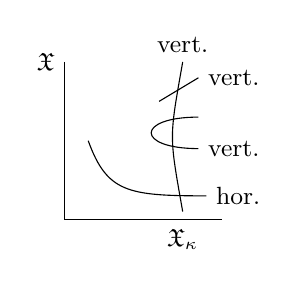
\begin{tikzpicture}[every node/.style={font=\small}]
			\draw (0,2) node[left] {$\mathfrak{X}$} -- (0,0) -- (2,0);
			\draw (1.5,2) node[above] {vert.} to[controls=+(260:1) and +(100:1)] (1.5,.1);
			\draw (1.2,1.5) -- (1.7,1.8) node[right] {vert.};
			\draw (1.7,1.3) to [controls=+(180:.8) and +(180:.8)] (1.7,0.9) node[right] {vert.};
			\draw (.3,1) to[controls=+(290:.7) and +(180:1)] (1.8,.3) node[right] {hor.};
			\path (1.5,0) node[below] {$\mathfrak{X}_{\kappa}$};
		\end{tikzpicture}
	\end{center}
\end{figure}

Let $E = \sum_{i=1}^{n} a_{i}E_{i}$ be a vertical divisor, and $D$ any divisor.
The intersection product is defined as:
\[
	(D \cdot E) = \sum_{i=1}^{n} a_{i} \deg \mathcal{O}(D)|_{\tilde{E_{i}}},
\]
where $\tilde{E_{i}} \to E_{i}$ is the normalisation.

The intersection product has the following properties:
\begin{itemize}
	\item It coincides with the geometric intuition if $D$ and $E$ have no common components.
	\item It is bilinear.
	\item It is symmetric if $D$ is vertical.
	\item It is invariant under linear equivalence on $D$.
	\item It is \emph{not(!)} invariant under linear equivalence on $E$.
		For example $\mathfrak{X}_{k} \sim 0$, but $(D \cdot
		\mathfrak{X}_{k}) \ne 0$ if $D$ consists of one horizontal
		component. See for example \cref{horvertdivs}.
	\item Behaviour under morphisms: If $h \colon \mathfrak{Y} \to
		\mathfrak{X}$ is a morphism of models, then
		\begin{center}
			\begin{tabular}{ll}
				$(D \cdot h^{*}E) = (h_{*}D \cdot E)$ &
				$(h^{*}D \cdot E) = (D \cdot h_{*}E)$ \\
				$D$ on $\mathfrak{Y}$ & $D$ on $\mathfrak{X}$ \\
				$E$ vertical on $\mathfrak{X}$ & $E$ vertical on $\mathfrak{Y}$
			\end{tabular}
		\end{center}
		which also imply $(h^{*}D \cdot h^{*}E) = (D \cdot E)$, when
		$D$ is a divisor on $\mathfrak{X}$, and $E$ a vertical divisor
		on $\mathfrak{X}$.
\end{itemize}

If $D$ is a divisor on a regular model $\mathcal{X}$ of $X$, then 
\[
(D \cdot \mathcal{X}_{k}) = \mathrm{deg}(D|_{X}).
\]
\begin{exercise}
	Prove this.
\end{exercise}

\section{Lecture 2}

\subsection{Minimal models}

A regular/nc/snc model $\mathfrak{X}$ of $X$ is called \emph{relatively
minimal} if every morphism of regular models $\mathfrak{X} \to \mathfrak{Y}$ is
an isomorphism. It is called \emph{minimal} if for all regular models
$\mathfrak{Y}$ there is a unique morphism of models $\mathfrak{Y} \to
\mathfrak{X}$.
\begin{example}
	$\mathbb{P}^{1}_{R}$ is a relatively minimal regular (even snc) model
	of $\mathbb{P}^{1}_{K}$, but it is \emph{not} minimal. The morphism
	$\phi \colon \mathbb{P}^{1}_{K} \to \mathbb{P}^{1}_{K}, (x : y) \mapsto
	(x : ty)$ does not extend to a morphism $\mathbb{P}^{1}_{R} \to
	\mathbb{P}^{1}_{R}$. So there does not exist morphism of regular models
	$\mathfrak{X} \to \mathbb{P}^{1}_{R}$, where $\mathfrak{X}$ is the
	model $\mathfrak{X} = \mathbb{P}^{1}_{R}$, $\mathfrak{X}_{K}
	\stackrel{\phi^{-1}}{\longrightarrow} \mathbb{P}^{1}_{K}$.

	However, one can show that $\mathfrak{X} = \mathbb{P}^{1}_{R}$ for
	\emph{every} relatively minimal regular model $\mathfrak{X}$.
\end{example}

\begin{proposition}
	$X$ always has a relatively minimal regular/nc/snc model.
	\begin{proof}
		Let $\mathfrak{X}$ be any regular/nc/snc model. If it is not
		relatively minimal, there is a map $\mathfrak{X} \to
		\mathfrak{Y}$ that is not an isomorphism. Such a map contracts
		a curve in the special fibre; but there are only finitely many
		of such curves.
	\end{proof}
\end{proposition}

\subsection{Important tools}

Any two regular/nc/snc can be dominated by a third such model.

\begin{theorem}[Factorisation theorem, Lichtenbaum, 1968]
	Every morphism of regular models is a finite composition of blow-ups at
	points centered in the special fibre.
\end{theorem}

\begin{theorem}[Castelnuovo's criterion, Lichtenbaum, 1968]
	Let $\mathfrak{X}$ be a regular model of $X$. Let $E$ be a vertical
	prime divisor on $X$. Then there exists a morpism of regular models $h
	\colon \mathfrak{X} \to \mathfrak{Y}$ such that $h(E) = \{y\}$ ($y$ a
	closed point) and such that $h$ is an isomorphism outside $E$ if and
	only if $E \cong \mathbb{P}^{1}_{k}$ and $(E \cdot E) = -1$. In that
	case, $h$ is the blow-up of $\mathfrak{Y}$ at $y$ and $E$ is called
	\emph{exceptional} on $\mathfrak{X}$.
\end{theorem}

\begin{exercise}
	If $g(X) \ge 1$, then $X$ has a (automatically unique) minimal
	regular/nc/snc model.
	\begin{solution}
		TODO
	\end{solution}
\end{exercise}

\subsection{Dual graph of an nc-model}

Let $\mathfrak{X}$ be any nc-model of $X$. Then the combinatorial properties of
$\mathfrak{X}_{k}$ are encoded in the \emph{dual graph}
$\Gamma(\mathfrak{X}_{k})$ of $\mathfrak{X}_{k}$. Write $\mathfrak{X}_{k}$ as
sum $\sum_{i \in I}N_{i}E_{i}$ of its irreducible components. Then
$\Gamma(\mathfrak{X}_{k})$ is a finite graph with vertices $\{ v_{i} | i \in I
\}$.
\begin{align*}
	\{\text{vertices } v_{i}\} &\longleftrightarrow \{ \text{irred. comps. of $\mathfrak{X}_{k}$} \} \\
	\{\text{loops at } v_{i}\} &\longleftrightarrow \{ \text{self-intersections of $E_{i}$} \} \\
	\{\text{edges} \} &\longleftrightarrow \{ \text{intersection points} \}
\end{align*}

\begin{center}
	\begin{tikzpicture}[every node/.style={font=\small}]
		\draw (0,0) -- (0,2) node[above] {$E_{1}$};
		\draw (-.3,.7) to [controls=+(40:3) and +(235:3)] (1,2) node[right] {$E_{2}$};
		\draw (-.3,.5) -- (1,.5) node[right] {$E_{3}$};
		\draw (-.3,.2) -- (1,.2) node[below] {$E_{4}$};
		\path (-.5,1.5) node {$\mathfrak{X}_{\kappa}$};

		\begin{scope}[xshift=6cm,yshift=1cm]
			\draw[fill] (0,0)  circle (0.01) node[left]  {$v_{1}$};
			\draw[fill] (1,1)  circle (0.01) node[right] {$v_{2}$};
			\draw[fill] (1,0)  circle (0.01) node[right] {$v_{3}$};
			\draw[fill] (1,-1) circle (0.01) node[right] {$v_{4}$};
			\draw (0,0) -- (1,1);
			\draw (1,1) to [controls=+(165:1) and +(90:1)] (1,1);
			\draw (0,0) -- (1,0);
			\draw (0,0) -- (1,-1);
			\path (-.5,.8) node {$\Gamma(\mathfrak{X}_{\kappa})$};
		\end{scope}
	\end{tikzpicture}
\end{center}

We label each vertex $v_{i}$ with the additional data $(N_{i}, p_{\textrm{a}}(E_{i}))$.

It is natural to ask which graphs can occur as dual graphs. There is one
immediate obstruction, which follows from the observation that for all $i \in
I$:
\begin{align*}
	0 &= \big(\sum_{j \in I} N_{j}E_{j} \cdot E_{i}\big) &&\text{by linear equivalence} \\
	&= \sum_{j \in I} N_{j} (E_{j} \cdot E_{i}) \\
	&= \sum_{j \ne i} N_{j} \underbrace{(E_{j} \cdot E_{i})}_{\parbox{4.5em}{\tiny \centering number of edges between $v_{i}$ and $v_{j}$}} + N_{i}(E_{i} \cdot E_{i})
\end{align*}
Consequently $\sum_{j \ne i} N_{j} (E_{j} \cdot E_{i})$ should be divisible by $N_{i}$.
\begin{theorem}[Winters]
	If for all $i \in I$, the sum $\sum_{j \ne i} N_{j} (E_{j} \cdot
	E_{i})$ is divisible by $N_{i}$, and $\gcd(N_{i}, i \in I) = 1$; then
	$\Gamma$ is a dual graph of an nc-model of a smooth projective
	geometrically connected curve $X$.

	The genera of the components $E_i$ can be chosen freely, modulo two
	conditions:
	\begin{itemize}
		\item the geometric genus $g$ satisfies $g \geq 0$,
		\item the arithmetic genus $p_a$ satisfies
			\[
				p_a \geq \#\{\text{self-intersection points}\}
				= \#\{\text{loops at a vertex}\}.
			\]
	\end{itemize}
\end{theorem}

\section{Lecture 3}
\input{lecture04.tex}
\input{lecture05.tex}
\section{Lecture 6}
\section{Lecture 7}


\begin{notation}
\hfill\\
$R$: complete DVR\\
$t$: uniformizer\\
$K$: quotient field\\
$k=k^{a}$: residue field
\end{notation}

We denote by $v_{K}$ the discrete valuation $K^{*}\rightarrow\ZZ$ and by $|\cdot|_{K}$ an absolute value on $K$:
\begin{align*}
K&\rightarrow\mathbb{R}^{+}\\
x&\mapsto
  \left\{
      \begin{aligned}
          &\exp(-v_{K}(x)) \; &\text{if} \; x\neq 0\\
          &0 \; &\text{if} \; x=0
      \end{aligned}
  \right.
\end{align*}

We use this structure on $K$ to develop a theory of analytic space over $K$ and in particular, to put an analytic structure
on algebraic varieties (just like over $\CC$).

Naive definition of analytic functions over $K$ (i.e., function locally given by converging power series) does not have
good properties because $k$ is totally disconnected with respect to the metric topology, e.g.
\begin{align*}
f:k&\rightarrow\mathbb{R}\\
x&\mapsto
  \left\{
      \begin{aligned}
          &1 \; &\text{if} \; x\in K\\
          &0 \; &\text{otherwise}
      \end{aligned}
  \right.
\end{align*}

We will use the theory developed by Berkovich at the end of the 80's.
We will only consider analytic spaces associated with algebraic varieties over $K$.

Let $X$ denote a scheme of finite type over $K$, then we define its Berkovich analytification as follows.
\begin{multline*}
X^{\mathrm{an}}:=\{x=(\xi_{x},|\cdot|_{x})\mid \xi_{x}\in X,\; |\cdot|_{x} \; \text{is an absolute value
on}\; \\ \kappa(\xi_{x}) \; \text{extending}\; |\cdot|_{K}\}
\end{multline*}
Then the following two properties are satisfied.
\begin{itemize}
  \item [(1)] the topology on $X^{\mathrm{an}}$ is finer than the Zariski topology on $X$, that is, the map
        $i:X^{\mathrm{an}}\rightarrow X: x=(\xi_{x},|\cdot|_{x})\mapsto\xi_{x}$ is continuous;
  \item [(2)] absolute value of regular functions are continuous, i.e., for every Zariski-open subset $U$ and
        every regular function $f\in\mathcal{O}_{X}(U)$, the map
        \[ |f|:i^{-1}(U)\rightarrow\mathbb{R}^{+}:x=(\xi_{x},|\cdot|_{x})\mapsto |f(x)|:=|f(\xi_{x})|_{x} \]
        is continuous.
\end{itemize}

If $x(=(\xi_{x},|\cdot|_{x}))\in X^{\mathrm{an}}$, then we can define the residue field $\mathscr{H}(x)$ of $X^{\mathrm{an}}$ at $x$
as the completion of $\kappa(\xi_{x})$ with respect to the absolute value $|\cdot|_{x}$. The field $\mathscr{H}(x)$
is a valued extension of $K$.
\begin{itemize}
  \item $\mathscr{H}(x)^{\circ}$=valuation ring ($|\cdot|_{x}\leq 1$)
  \item $\mathscr{H}(x)^{\circ\circ}$=maximal ideal ($|\cdot|_{x}< 1$)
  \item $\widetilde{\mathscr{H}(x)}$=residue field=$\mathscr{H}(x)^{\circ}/\mathscr{H}(x)^{\circ\circ}$
\end{itemize}

Then we have the following topological properties of $X^{\mathrm{an}}$.
\begin{itemize}
  \item [(1)] $X^{\mathrm{an}}$ is locally compact and locally path-connected.
  \item [(2)] $X^{\mathrm{an}}$ is connected $\Leftrightarrow$ $X$ is connected.
  \item [(3)] $X^{\mathrm{an}}$ is Hausdorff $\Leftrightarrow$ $X$ is separated.
  \item [(4)] $X^{\mathrm{an}}$ is compact $\Leftrightarrow$ $X$ is proper.
\end{itemize}

We also notice that
\begin{itemize}
  \item If $\xi$ is a closed point of $X$, then $i^{-1}(\xi)=\{(\xi,|\cdot|)\}$ is a
        unique extension of $|\cdot|_{K}$ to $\kappa(\xi)$ which is a finite extension of $K$.
  \item If $\xi$ is not closed, then $i^{-1}(\xi)$ is nonempty and in fact, very large.
\end{itemize}

If $X$ is integral, we consider
\begin{eqnarray*}
X^{\mathrm{an}}\supset i^{-1}(\eta_{x})=
\left\{
\text{absolute value on} \scriptstyle \atop
K(X) \;\text{extending} \; |\cdot|_{K}
\right\}
&\longleftrightarrow &
\left\{
\text{real valuation} \; K(X)^{*}\rightarrow\mathbb{R} \scriptstyle \atop
\text{extending} \; v_{K}
\right\}^{X}\\
|\cdot|&\mapsto &-\ln|\cdot|\\
\exp(-v(\cdot))&\leftmapsto &v(\cdot)
\end{eqnarray*}
The latter is classically studied in birational geometry.

\begin{observation}
It is (very) difficult to understand the geometry of $X^{\mathrm{an}}$ directly from the definition
if $\mathrm{dim}(X)\geq 2$.
\end{observation}
So we will analyze the structure using the geometry of models.

\section{Lecture 8}

We will assume from now on that $X$ is a smooth, proper and geometrically connected curve.

Let $\mathscr{X}$ be an $snc$-model of $X$ over $R$. Then we can use $\mathscr{X}$ to produce an interesting set of
points in $X^{\mathrm{bir}}\subset X^{\mathrm{an}}$ which we call the divisorial points.
Here $X^{\mathrm{bir}}$ denotes the set of birational points
of $X^{\mathrm{an}}$.

Write the special fiber as $\mathscr{X}_{k}=\sum_{i\in I}N_{i}E_{i}$, we consider the valuation
\[
  v: \kappa(x)^{*}\rightarrow\mathbb{R}: f\mapsto \frac{1}{N_{i}}\mathrm{ord}_{E_{i}}f
\]
such that $v(t)=1$. In fact, this $v$ extends the valuation $v_{K}$ on $K$ and
gives rise to a point $x\in X^{\mathrm{an}}$ which we call the divisorial point associated with
$(\mathscr{X},E_{i})$.

\begin{exercise}
Compute $\mathscr{H}(x)$.
\end{exercise}

We say that a point of $X^{\mathrm{an}}$ is divisorial if it is the divisorial point associated with some
$snc$-model $\mathscr{X}$ and some component of $\mathscr{X}_{k}$.

\begin{fact}
The set of divisorial points in $X^{\mathrm{an}}$ is dense, but the induced topology on this set is totally disconnected.
\end{fact}
We can glue them together by interpolations of monomial points.

\begin{proposition}
Let $\mathscr{X}$ be an $snc$-model of $X$, write $\mathscr{X}_{k}=\sum_{i\in I}N_{i}E_{i}$. Let $x$ be an intersection
point of $E_{i}$ and $E_{j}$ with $i\neq j$, take $\alpha_{i},\alpha_{j}\in\mathbb{R}^{+}$ such that
$\alpha_{i}N_{i}+\alpha_{j}N_{j}=1$. Then there exists a unique smallest valuation
\[
   v:\mathcal{O}_{X,x}\backslash\{0\}\rightarrow\mathbb{R}^{+}
\]
such that $v(z_{i})=\alpha_{i},v(z_{j})=\alpha_{j}$, where $z_{i},z_{j}$ are local equations for $E_{i},E_{j}$
at $x$.
\end{proposition}

We will sketch the construction of such a valuation $v$. For $R=k[[t]]$, we have $\hat{\mathcal{O}}_{X,x}\cong k[[z_{i},
z_{j}]]$. It is not difficult to show that every element $f\in\mathcal{O}_{X,x}\backslash\{0\}$ can be written
in the completed local ring $\hat{\mathcal{O}}_{X,x}$ as a power series
\[ f=\sum_{\beta\in\mathbb{N}^{\{i,j\}}}c_{\beta}z_{i}^{\beta_{i}}z_{j}^{\beta_{j}} \]
where each coefficient $c_{\beta}\in k$. Then
\[ v(f)=\mathrm{min}\{\alpha_{i}\beta_{i}+\alpha_{j}\beta_{j}\mid\beta\in\mathbb{N}^{\{i,j\}},c_{\beta}\neq 0\}. \]
This valuation $v$ extends to a real valuation $v:K(X)^{*}\rightarrow\mathbb{R}$ such that
$v(t)=v(\mathrm{unit}.z_{i}^{N_{i}}z_{j}^{N_{j}})=N_{i}\alpha_{i}+N_{j}\alpha_{j}=1$. Thus $v$ extends
$v_{K}$ on $K$ and therefore gives rise to a point $y\in X^{\mathrm{an}}$ which we call the monomial point
associated with $(\mathscr{X},(E_{i},E_{j}),(\alpha_{i},\alpha_{j}),x)$.

\begin{exercise}
  \begin{enumerate}
    \item For $\alpha_{i}=1/N_{i},\alpha_{j}=0$, then $y$ is the divisorial point associated with $(\mathscr{X},E_{i})$.
    \item Show that $y$ is still monomial with respect to the blow up of $\mathscr{X}$ at $x$ and determines
          the associated components and parameter vector $\alpha$.
    \item Show that $y$ is divisorial if and only if $\alpha_{i},\alpha_{j}\in\mathbb{Q}$.
  \end{enumerate}
\end{exercise}

\begin{definition}
If $\mathscr{X}$ is an $snc$-model of $X$, then the Berkovich skeleton $\mathrm{Sk}(\mathscr{X})$ is the set
of $y\in X^{\mathrm{an}}$ that are monomial with respect to $\mathscr{X}$.
\end{definition}

We will now construct a map as follows.
\begin{eqnarray*}
\Phi:\Gamma(\mathscr{X}_{k}) &\rightarrow &\mathrm{Sk}(\mathscr{X})\\
\left\{
\begin{array}{@{}c@{}}
\text{vertex} \; v_{i} \\
\updownarrow \\
\text{component}\; E_{i} \; \text{in} \; \mathscr{X}_{k}
\end{array}
\right\}
&\mapsto &
\left\{
\begin{array}{@{}c@{}}
\text{divisorial point} \\
\text{associated with} \; (\mathscr{X},E_{i})
\end{array}
\right\}\\
\left\{
\begin{array}{@{}c@{}}
\text{point with barycentric} \\
\text{coordinate} \; (\lambda_{i},\lambda_{j}) \\
\text{on an edge} \; e_{x} \\
\text{corresponding to}\; x\in E_{i}\cap E_{j}
\end{array}
\right\}
&\mapsto &
\left\{
\begin{array}{@{}c@{}}
\text{monomial point associated} \\
\text{with} \; (\mathscr{X},(E_{i},E_{j}),(\frac{\lambda_{i}}{N_{i}},\frac{\lambda_{j}}{N_{j}}),x)
\end{array}
\right\}
\end{eqnarray*}

\begin{proposition}
The map $\Phi$ is a homeomorphism.
\end{proposition}

\begin{proof}
It is not hard to see that $\Phi$ is a bijection. (exercise)

It is continuous. (exercise)

Then we have that it is a homeomorphism since $\Gamma(\mathscr{X}_{k})$ is compact and $\mathrm{Sk}(\mathscr{X})$ is
Hausdorff.
\end{proof}

\begin{proposition}
The embedding $\mathrm{Sk}(\mathscr{X})\hookrightarrow X^{\mathrm{an}}$ has a canonical retraction
\[ \rho_{\mathscr{X}}:X^{\mathrm{an}}\rightarrow\mathrm{Sk}(\mathscr{X}). \]
\end{proposition}

The construction takes two steps. The first step is to construct the specialization map as follows
\begin{align*}
\mathrm{sp}_{\mathscr{X}}:X^{\mathrm{an}}&\rightarrow \mathscr{X}_{k} \\
x&\mapsto
\left\{
\text{the image of the closed point of} \; \Spec\mathscr{H}(x)^{\circ} \scriptstyle \atop
\text{under} \; \Spec\mathscr{H}(x)^{\circ}\rightarrow\mathscr{X}
\right\}
\end{align*}
Since $\mathscr{X}$ is proper over $R$, the canonical morphism $\Spec\mathscr{H}(x)\rightarrow X\hookrightarrow
\mathscr{X}$ can be uniquely extended to a morphism $\Spec\mathscr{H}(x)^{\circ}\rightarrow\mathscr{X}$ by the
valuative criterion of separatedness.

\begin{example}
$x\in X(K)$ extends to $\Spec R\rightarrow \mathscr{X}$ and reduction mod $t$ yields
$(\Spec k\rightarrow\mathscr{X}_{k})=\mathrm{sp}_{\mathscr{X}}(x)$.
\end{example}

\begin{exercise}
(1) Show that $\mathrm{sp}_{\mathscr{X}}$ is anticoutinuous. (i.e., inverse image of a closed set is open.)

(2) If $y$ is a monomial point associated with $(\mathscr{X},(E_{i},E_{j}),(\alpha_{i},\alpha_{j}),x)$.
Assume $\alpha_{i},\alpha_{j}\neq 0$, show that $\mathrm{sp}_{\mathscr{X}}(y)=x$.
\end{exercise}

Now $\rho_{\mathscr{X}}$ can be defined as follows.
\begin{itemize}
  \item If $\mathrm{sp}_{\mathscr{X}}(x)$ lies on a unique component $E_{i}$, then
        $\rho_{\mathscr{X}}(x):=\text{divisorial}$ point associated with $(\mathscr{X},E_{i})$;
  \item If $\mathrm{sp}_{\mathscr{X}}(x)\in E_{i}\cap E_{j}$ for $i\neq j$, then
        $\rho_{\mathscr{X}}(x):=\text{monomial point associated with}$
        $(\mathscr{X},(E_{i},E_{j}),(-\ln|z_{i}(x)|,-\ln|z_{j}(x)|),\mathrm{sp}_{\mathscr{X}}(x))$, where
        $z_{i},z_{j}$ are local equations for $E_{i},E_{j}$ at $\mathrm{sp}_{\mathscr{X}}(x)$.
\end{itemize}

\begin{exercise}
Show that $\rho_{\mathscr{X}}$ is continuous.
\end{exercise}

\section{Understanding how line bundles degenerate (Lecture 9)}

Let $A$ be an abelian variety over $K$ and assume $K=\CC((t))$.

\begin{definition} A N\'eron model of $A$ is a smooth and separated $R$-scheme $A_{R}$ with the property that for any smooth and separated $X/R$ and any morphism $X_K\to A_K$ there is a unique extension $X_R\to A_R$. \end{definition}

In particular $A_R(R) = A(K)$

\begin{theorem} A N\'eron model exists and is a commutative group scheme over $R$, N\'eron, Raynaud\end{theorem}
\begin{proof} See N\'eron models by Bosch, L\"utkebohmert, Raynaud. \end{proof}

\noindent When $A=\Jac(X)$ the special fiber of a N\'eron model is the smooth locus in the special fiber of Caporaso's relative compactified Jacobian. (This represents a "balanced" Picard functor).

We will consider the special case where $X$ is a curve with a regular semistable snc model $\mathfrak{X}$ over $R$. Let $G$ be the dual graph of $\mathfrak{X}$. Our goal will be to understand how line bundles of degree 0 degenerate.

\noindent Maximal torus: the line bundles that are trivial on each component of $\overline{\mathfrak{X}}$.

\[\text{Maximal torus} \subseteq \text{Conn. component of the identity} \subseteq A\twoheadrightarrow \text{Component group}\]

%TODO: image of two tori attached to a sphere and a graph depicting a triangle as its model

\[\text{Line bundles on }\overline{\mathfrak{X}}\text{ trivial on each component} \longleftrightarrow \Hom(\pi_1(G),\CC^*) = \Hom(H_1(G,\ZZ),\CC^*)\]

\[\text{Special fiber of N\'eron model}\to \prod_i \Pic(\overline{\mathfrak{X}_i})\]

\noindent The kernel of 

\[\text{Conn. component of the identity}\to \prod_i \Jac(\overline{\mathfrak{X}_i})\] is the maximal torus of rank = $h^1(G)$.

\noindent The component group of $A_{\CC}$ is the obstruction to extending a line bundle of degree 0 on $X$ to a line bundle of degree 0 on each $\overline{\mathfrak{X}_i}$.

\noindent Obstruction = $\Jac(G)$.

The identification of $\Jac(G)$ with the component group of $A_{\CC}$ induces an inclusion $\Jac(G)\hookrightarrow \Jac(X)^{\an}$.

A component $y$ of $A_{\CC}$ gives rise to a valuation $\ord_y$ on $K(A)$ and since $A_R$ is smooth over $\Spec R$ each component is reduced and $\ord_y$ extends to a valuation on $K$.

%TODO image of a Torus A degenerating into several connected components in A_{\CC}

\[
	A_K^{\an} = \left\{(\mathfrak{p},\val) \middle\vert
		\parbox{.5\textwidth}{\centering$\mathfrak{p}\in A$ and $\val$ is a valuation on $\mathcal{K}(\mathfrak{p})$ that extends the valuation on $K$.}
	\right\}
\]

\[\Jac(G)\subset \Jac(X)^{\an}\]

To get more information, we can extend the field. Let $L|K$ be a finite extension, so $L = \CC((t^{\frac{1}{n}}))$. This gives rise to a curve $X_L$ and a model $\mathfrak{X}_L$ which is a resolution of $\mathfrak{X}\times_R R_L$. The dual graph of $\overline{\mathfrak{X}_L}$ is $\frac{1}{N}(G)$.

Now build a N\'eron model of $\Jac(X_L)$. The component group of the special fiber is $\Jac(\frac{1}{N}(G))$.

\[
\xymatrix{
X_L \ar[d] & \Jac(X_L) \ar[d] \ar@{~>}[r] & \Jac(X_L)_{\CC} \\
X_K & \Jac(X_K) \ar@{~>}[r] & \Jac(X_K)_{\CC}
}
\]
%TODO: The arrowheads on the squigly arrows look weird.

\noindent We can pull rational functions on $\Jac(X_K)$ back  to to $\Jac(X_L)$ and get $\ord_y$ for $y\in\Jac(\frac{1}{N}G$. Now $\frac{1}{N}\ord_y$ extends the valuation on $K$. (We divide by $N$ to remove the ramification). With this we also get that $\Jac(\frac{1}{N})$ is included in $\Jac(X)^{\an}$.

\begin{definition} We define the skeleton $\Sigma(\Jac(X_K)^{\an})$ to be $\overline{\bigcup_N \Jac(\frac{1}{N}G)}$.
\end{definition}

\input{lecture10.tex}
\section{Lecture 11}
\section{Lecture 12}
\section{Lecture 13}
\section{ Mumford uniformization (Lecture 14)}

\noindent Let $X$ be a smooth projective curve of genus $g$ over $K=\CC((t))$ and let $\mathfrak{X}$ be a regular semistable snc model. Furthermore set $R = \CC[[t]]$. Now $\overline{\mathfrak{X}}$ is a union of $\mathbb{P}^1$ s, so $h^1(G) = g$.

Last time we saw that $\Jac(G)_{\RR} = \Hom(H_1(G),\RR)/H_1(G,\ZZ)$ where $H_1(G,\ZZ)\subset \Hom(H_1(G),\ZZ)\subset \Hom(H_1(G),\RR)$ is induced by $<,>$. We also saw that the maximal torus $T$ in $\overline{\Pic(\mathfrak{X}/R)}$ is equal to the identity component and is $\Hom(H_1(G),\CC^*)$. So $T$ is an algebraic torus with character lattice $M = H_1(G,\ZZ)$. Set $N=M^{\vee}$.

\begin{theorem} (Mumford uniformization) $\Jac(X)^{\an} = T_K^{\an}/H_1(G,\ZZ)$. \end{theorem}

\noindent For each $x\in T(K)$ we can get a map 

\[
\xymatrix{
M \ar[r]^{\mathrm{ev}_{x}} & K^*  \ar[r]^{\val} & \RR \\
}
\]

which determines a group homomorphism $T(K)\to N_{\RR}$. We can say in some sense that $\Trop(x)\in N_{\RR}$.

\noindent Now if $L|K$ is a valued extension and $y\in T(L)$ we can also get a map

\[
\xymatrix{
M \ar[r]^{\mathrm{ev}_{y}} & L^*  \ar[r]^{\mathrm{val}} & \RR \\
}
\]

\noindent If $y$ were defined over $K$ we'd get the same map. Using this we get compatible maps $T(L)\to N_{\RR}$ for all valued extensions $L|K$.

\noindent If $Y$ is a variety over $K$, an alternative description of $Y^{\an}$ is the set

$Y^{\an}=\{y\in Y(L)$ for valued extensions $L|K \}$

modulo an equivalence relation: We say that $(y,L)\sim (y',L')$ if there exists a pair $(y'',L'')$ such that $L\subseteq L''$, $L'\subset L''$ and $y''=y\times_{L} L'' = y'\times_L L''$.

\noindent Combining these things we end up with a surjective map $\pi: T^{\an}\twoheadrightarrow N_{\RR}$.

\noindent We also need an injective map $N_{\RR}\hookrightarrow T^{\an}$. 

Given $v\in N_{\RR}$ we want to give a valuation. Define $\val_v(f) = \min_{x\in \pi^{-1}(v)}\val_x(f)$.
\noindent These are all monomial valuations. Another way of describing the valuation is 

\[\val_v(\sum_{u\in M \text{ finite }}a_{u}X^u) = \min_u\{\val(a_u)+<u,v>\}\]

$\pi^{-1}(0)$ is a compact analytic subgroup of $T^{\an}$ which we call $T_0$. 

$T_0(L) = T(R_L)$

\noindent We can now see that we more or less have that $N_{\RR} = T^{\an}/T_0$. This statement has been made more precise by the following theorem

\begin{theorem} $N_{\RR} = (T^{\an}/T_0)^{\an}$ (Abramovich--Chen--Markus--Wise)/Mulisch?

\noindent Rough picture. Good analogue of skeleton of a Jacobian.

\end{theorem}
 
\[
\xymatrix{
 & T^{\an} \ar@{->>}[r] \ar@{->>}[d]^{/T_0} & \Jac(X)^{\an} \ar[d]^{/T_0} \\
H_1(G,\ZZ) \ar@{^{(}->}[r] & \Hom(H_1(G),\RR) \ar[r] \ar@{=}[d] & \Jac(G)_{\RR} = N_{\RR}/H_1(G,\ZZ) \\
 & N_{\RR} = \Sigma(T^{\an}) \ar[r] & \Sigma(\Jac(X)^{\an}) 
 }
\]

References: 
Gubler: Tropicaliztion of analytic spaces (2006?)
Baker-Rabinoff (2013?)

\section{Lecture 15}

\end{document}
